\section{Data Processing}
This section covers processing of acquired data. All data processing is performed using MATLAB. 

%maybe something on filtering if we end up doing that
\subsection{Filtering} \label{subsec:filtering}
%Butterworth filtering of the gyroscope measurements
%Filtering has been implemented in the form of a low pass third order Butterworth filter with a cut off frequency at 25Hz. Since measurement are 
%In order to determine a adequate filter for filtering of the FSR data the a spectral analysis have been conducted. A Fourier transform (FT) of FSR data can be seen in \figref{fig:FSR_FFTplot}, where it can be seen that frequencies 

%The spectral density of gyroscope data have been analysed to investigate frequencies of interest. From the Fourier transform (FT) of gyroscope data (see \figref{fig:gyroFFTPlot}) it can be observed that frequencies over 10Hz contain very little information. To avoid possible noise and artefacts a low pass third order Butterworth filter have been implemented with a cut off frequency at 25Hz. %no

Acquired FSR data is filtered with a third order low pass Butterworth filter with cutoff at 5Hz, according to \cite{Prieto1996}. 
However, during the experiment it was observed that subjects dragged their feet over the ground when performing the kata. This was not anticipated, and an examination of acquired data showed noise artefacts in frequencies above 1Hz, associated with dragging the feet. As the goal for this study is to investigate subjects sway of balance during movements, and not directly determining movements, the cutoff frequency was changed to 2.5Hz. A cutoff at this frequency showed good results.

Gyroscope data have been filtered through a third order low pass Butterworth filter with cutoff frequency set at 1.25Hz, according to \cite{Alberts2015}. 

% figure is obsolete
%\begin{figure}[H] 
%	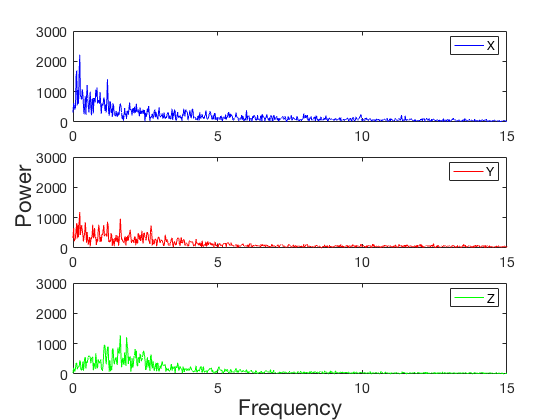
\includegraphics[width=.8\textwidth]{figures/gyroFFTPlot}
%	\caption{The power spectral density of gyroscope data from the left leg of one subject.}
%	\label{fig:gyroFFTPlot}  %<--remember LABEL!
%\end{figure}



%MATLAB alignment GUI description
\subsection{Data Alignment}
Because the measurements from the FSRs are run on an Arduino, and the gyroscopes run through a Shimmer Sensing developed script for MATLAB, the timing for the measurements are run differently. In order to analyse FSR data to the corresponding time for gyroscope data a data alignment GUI have been developed in MATLAB. The implemented alignment program is a simple GUI which creates a plot where different channels from the six FSRs and six DoFs from the gyroscopes (three for each on each leg) can be shown or hidden. Additionally each channel can be translated left or right. This enables to align data from the FSRs to the gyroscopes, based on a spike in measurements caused by a small jump subjects will be asked to perform before and after performance of Pinan Nidan. An example of the alignment GUI in work can be seen in \figref{fig:alignGUI}.

\begin{figure}[H]
	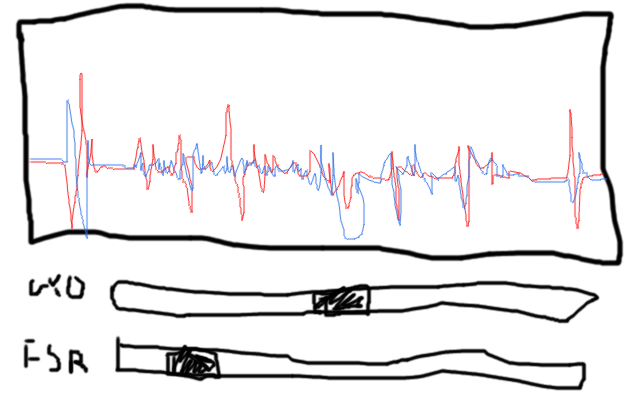
\includegraphics[width=1\textwidth]{figures/alignGUI}
	\caption{The alignment GUI showing a selected number of channels from the FSRs and gyroscopes. All channels can be translated in order to align timestamps for the FSR measurements to timestamps for the gyroscopes.}
	\label{fig:alignGUI}  %<--remember LABEL!
\end{figure}

